% Template for Part III essays 2024/25 (12.02.2025)
% Authors: Mycroft Rosca-Mead, Matt Colbrook, Jonathan Evans.

%%%%%%%%%%%%%%%%%%%%%%%%%%%%%%%%%%%%%%%%%%%%%%%%%%%%%%%%%%%%%%%%%%%%%%

% The following few lines are preliminaries and MUST NOT BE EDITED
\documentclass[11pt, titlepage]{article} % DO NOT CHANGE THE FONT SIZE
\usepackage[left=2.2cm,right=2.2cm,top=2.5cm,bottom=2.5cm]{geometry} % DO NOT CHANGE THE MARGINS
\usepackage{amsfonts,amssymb,amsthm,amsmath,amscd}
\usepackage{enumerate}
\usepackage{tikz}

%%%%%%%%%%%%%%%%%%%%%%%%%%%%%%%%%%%%%%%%%%%%%%%%%%%%%%%%%%%%%%%%%%%%%%

% ESSAY TITLE
% Your essay title should match the title given in the essay booklet.
% If you wish to give the essay your own subtitle, you can do this after the title page (e.g. using \section*{Subtitle Name}).
% You do not need to use \Author and YOU SHOULD NOT INCLUDE YOUR NAME OR COLLEGE ANYWHERE IN THIS ESSAY.
% The title page does not count towards the total page number.
\title{New Advances in Conformal Prediction}

% DATE
%To remove the date from the front page of the final version, UNCOMMENT the line below.
%\date{}

% FONTS
%\renewcommand{\familydefault}{\sfdefault}
% YOU MUST USE EITHER THE SANS-SERIF FONT DEFINED BY THE COMMAND ABOVE OR THE STANDARD LaTeX (computer modern) FONT THAT CAN BE OBTAINED BY COMMENTING OUT THE LINE ABOVE. YOU MUST NOT USE ANY OTHER FONT.

%%%%%%%%%%%%%%%%%%%%%%%%%%%%%%%%%%%%%%%%%%%%%%%%%%%%%%%%%%%%%%%%%%%%%%
% A guide to using LaTeX can be found online at https://www.overleaf.com/learn/latex/Learn_LaTeX_in_30_minutes.
% A shorter LaTeX cheat sheet can be found at https://wch.github.io/latexsheet/.

%%%%%%%%%%%%%%%%%%%%%%%%%%%%%%%%%%%%%%%%%%%%%%%%%%%%%%%%%%%%%%%%%%%%%%
% Some latex tips:

% Use this space for any special macros or packages you need.
\usepackage{graphicx}
\usepackage[backend=biber, sorting=none, style=alphabetic]{biblatex}
\addbibresource{refs.bib}

\usepackage{bbm}
\usepackage{algorithm}
\usepackage{algpseudocode}
\usepackage{caption}
\usepackage{subcaption}

\DeclareMathOperator*{\argmin}{argmin}

\renewcommand{\algorithmicrequire}{\textbf{Input:}}
\renewcommand{\algorithmicensure}{\textbf{Output:}}

\newcommand{\R}{\mathrm}
\newcommand{\B}{\mathbf}
\newcommand{\Prob}[1]{\mathbb{P}\left( #1 \right)}
\newcommand{\Exp}[3]{\mathbb{E}\left#2 #1 \right#3}
\newcommand{\Ind}[1]{\mathbbm{1}\left\{ #1 \right\}}

\usepackage{hyperref}
\usepackage{mathtools}
% use this package for easy referencing:
\usepackage[capitalise,noabbrev]{cleveref} % e.g., \cref{amazing_theorem} will reference "`Theorem"' X without having to keep track of theorems, equations etc and typing "`Theorem"'
\usepackage{overpic} % use this package for easy labelling of figures
\usepackage{url} % use this package to reference urls, e.g., \url{https://www.maths.cam.ac.uk/postgrad/part-iii/prospective.html}
\usepackage{comment} % use this package to comment things out \begin{comment} blah \end{comment}

% FIGURES
% Here is an example of how to do figures:

%\begin{figure}
%\centering
%\includegraphics[width=\linewidth]{CMS at night_0.jpg}
%\caption{The CMS at night.}\label{fig:cms}
%\end{figure}

% General tip: Many tex problems can be easily solved by a quick and specific google search.


%%%%%%%%%%%%%%%%%%%%%%%%%%%%%%%%%%%%%%%%%%%%%%%%%%%%%%%%%%%%%%%%%%%%%%
%FOOTNOTES
\newcommand\blfootnote[1]{% avoids footnotes spilling over
  \begingroup
  \renewcommand\thefootnote{}\footnote{#1}%
  \addtocounter{footnote}{-1}%
  \endgroup
}

%%%%%%%%%%%%%%%%%%%%%%%%%%%%%%%%%%%%%%%%%%%%%%%%%%%%%%%%%%%%%%%%%%%%%%
% The following relate to equations, theorems, etc, as illustarted in the document. 

\numberwithin{equation}{section}
% EQUATION NUMBERING: The command above can be changed to number equations within subsections, rather than sections, or it can be commented out to number equations through the document, irrespective of (sub)sections.

\newtheorem{theorem}{Theorem}
\newtheorem{lemma}{Lemma}
\newtheorem{corollary}{Corollary}
\newtheorem{proposition}{Proposition}
\theoremstyle{definition}
\newtheorem{definition}{Definition}
\newtheorem{remark}{Remark}
\newtheorem{example}{Example}

\numberwithin{theorem}{section}
\numberwithin{lemma}{section}
\numberwithin{corollary}{section}
\numberwithin{proposition}{section}
\numberwithin{definition}{section}
\numberwithin{remark}{section}
% NUMBERING OF THEOREMS ETC: The commands above can be changed to number within subsections, rather than sections, or commented out to number them through the document, irrespective of (sub)sections.

%%%%%%%%%%%%%%%%%%%%%%%%%%%%%%%%%%%%%%%%%%%%%%%%%%%%%%%%%%%%%%%%%%%%%%
\begin{document}
\maketitle
%%%%%%%%%%%%%%%%%%%%%%%%%%%%%%%%%%%%%%%%%%%%%%%%%%%%%%%%%%%%%%%%%%%%%%

% START WRITING YOUR ESSAY HERE

\section{Introduction}
\subsection{Notation}





\label{sec:intro}

\section{Foundations of Conformal Prediction}
\label{sec:foundations_of_CP}

The primary appeal of conformal prediction, as originally developed by Vovk et. al. \cite{vovk2005algorithmic}, lies in the fact that the coverage guarantee holds in a distribution-free sense and in finite samples. Compare this to the construction of prediction sets in classical statistics, which often relies on strong distributional assumptions (such as normality) and may only hold asymptotically. \vskip 5pt

\noindent
In this chapter, we develop the mathematical foundations of conformal prediction. We begin by defining the key concepts of quantiles, empirical cumulative distribution functions and exchangeability in \cref{subsec:quantiles_and_exchangeability}. In sections \cref{subsec:fullconformal} and \cref{subsec:splitconformal}, we present the two main variants of conformal prediction: full conformal prediction and split conformal prediction, respectively, and prove their coverage guarantees. In \cref{subsec:conformityscore}, we consider specific instances of conformal prediction and compare these through numerical experiments.

\subsection{Quantiles and exchangeability}
\label{subsec:quantiles_and_exchangeability}

In the following definitions, we introduce the notions of quantiles, empirical cumulative distribution functions and exchangeability, which are fundamental to conformal prediction. The results in this subsection are stated as facts in \cite{angelopoulos2024theoreticalfoundationsconformalprediction}, and we provide our own proofs for these. The proof of \cref{lemma:exch_cdfquantile} follows the proof of Lemma 1 in \cite{romano2019_CQR}.

\begin{definition}[Exchangeability]
    The random variables \(Z_1, ..., Z_n\) are exchangeable if for all \(\sigma \in S_n\), we have that \[(Z_1, \ldots, Z_n) \overset{d}{=} (Z_{\sigma(1)}, \ldots, Z_{\sigma(n)}).\] Equivalently, \(Z_1, ..., Z_n\) are exchangeable if for any measurable set \(A\) and for any \(\sigma \in S_n\), we have that \[\Prob{(X_1, \ldots, X_n) \in A} = \Prob{(X_{\sigma(1)}, \ldots, X_{\sigma(n)}}) \in A.\]
\label{defn:exch}
\end{definition}

\begin{remark}
Note that if \(Z_1, \ldots, Z_n\) are exchangeable random variables taking values in \(\mathcal{Z}\), then they must be identically distributed. Indeed, for any measurable set \(A \in \mathcal{Z}\) and \(i \in [n]\), we have that \begin{align*} 
    \Prob{Z_i \in A} &= \Prob{(Z_1, \ldots, Z_{i-1}, Z_i, Z_{i+1} \ldots, Z_n) \in \mathcal{Z} \times \cdots \times \mathcal{Z} \times A \times \mathcal{Z} \times \ldots \times \mathcal{Z}} \\
    &= \Prob{(Z_i, \ldots, Z_{i-1}, Z_1, Z_{i+1} \ldots, Z_n) \in \mathcal{Z} \times \cdots \times \mathcal{Z} \times A \times \mathcal{Z} \times \ldots \times \mathcal{Z}} \\
    &= \Prob{Z_1 \in A},
\end{align*} where we use exchangeability to obtain the second equality. However, exchangeable random variables need not be independent. Indeed, if \(Z_1, \ldots, Z_n\) are sampled without replacement from the set \([n]\), then they are exchangeable, since any particular realisation has probability \(\frac{1}{n!}\), but \(Z_1, \ldots, Z_n\) are certainly not independent. Therefore, we see that exchangeability is a weaker condition that being i.i.d.
\label{rmk:exch_dist}
\end{remark}

\begin{remark}
    Another way to view exchangeability is as follows. Suppose the random variables \(Z_1, \ldots, Z_n \in \mathbb{R}\) are almost surely distinct and exchangeable. Taking \(A = \{(z_1, \ldots, z_n) \in \mathbb{R}^n : z_1 < z_2 < \cdots < z_n \}\), we have that for any \(\sigma \in S_n\), \[\Prob{Z_1 < \cdots < Z_n} = \Prob{(Z_1, \ldots, Z_n) \in A} = \Prob{(Z_{\sigma(1)}, \ldots, Z_{\sigma(n)}) \in A} = \Prob{Z_{\sigma(1)} < \cdots < Z_{\sigma(n)}}.\] This means that \(Z_1, \ldots, Z_n\) are equally likely to appear in any given ordering.
\label{rmk:exch_ordering}
\end{remark}

\begin{definition}
    Let \(P\) be a probability distribution on \(\mathbb{R}\) with cumulative distribution function \(F\). The \textit{quantile function} of \(P\) is defined for \(\beta \in (0,1)\) by \[Q(P;\beta) \coloneqq \inf\left\{ z \in \mathbb{R}: F(z) \geq \beta \right\}.\] We may also use the notation \(Q(F;\beta)\) in place of \(Q(P;\beta)\).
\label{defn:prob_quantile}
\end{definition}

\begin{definition}
    For \(z \in \mathbb{R}^n\), we define the following quantities. \begin{enumerate}[(i)] \itemsep0em
        \item The \textit{empirical cumulative distribution function} of \(z\) is the function \(F_z: (-\infty, \infty] \to [0,1]\) given for \(x \in (0, \infty)\) by \[\hat{F}_z(x) \coloneqq \frac{1}{n}\sum_{i=1}^n \Ind{z_i \leq x}.  \] We define \(\hat{F}_z(\infty) = 1\).
        \item The \textit{quantile function} \(\hat{Q}_z:(0,1] \to (-\infty, \infty]\) of \(z\) is defined for \(\beta \in (0,1]\) by \[\hat{Q}_z(\beta) \coloneqq \inf \left\{ x \in (-\infty, \infty]: \hat{F}_z(x) \geq \beta \right\}.\]
    \end{enumerate}
\label{defn:empirical_cdfquantile}
\end{definition}

\begin{remark}
    Note that \(\hat{F}_z\) is the cumulative distribution function of the probability distribution \[\frac{1}{n} \sum_{i=1}^n \delta_{z_i},\] where \(\delta_{a}\) denotes the Dirac measure at \(a\), for any \(a \in \mathbb{R}\). We also have that \[\hat{Q}_z(\beta) = Q\left( \frac{1}{n}\sum_{i=1}^n \delta_{z_i} ; \, \beta \right),\] so \(\hat{Q}_z\) is the quantile function of the probability distribution \(\frac{1}{n} \sum_{i=1}^n \delta_{z_i}.\)
\end{remark}

\noindent
The following lemma formalises a sense in which the empirical cumulative distribution and quantile functions are inverses of each other.

\begin{lemma}
    Let \(z \in \mathbb{R}^n\) and \(\beta \in (0,1)\). Then we have that \(\hat{F}_z\left(\hat{Q}_z(\beta)\right) \geq \beta\). If, moreover, the components of \(z\) are distinct, then \(\hat{F}_z\left(\hat{Q}_z(\beta)\right) = \frac{\lceil{n\beta}\rceil}{n}.\)
\label{lemma:cdfquantile}
\end{lemma}
\begin{proof}
    The first claim follows from the definitions upon noting that \(\hat{F}_z\) is right-continuous. For the second claim, we observe that for all \(x \in \mathbb{R}\), we have that \(\hat{F}_z(x) \in \left\{0, \frac{1}{n}, \ldots, \frac{n-1}{n}, 1\right\}\). Since the components of \(z = (z_1, \ldots, z_n)\) are distinct, \(\hat{F}_z\) jumps by \(\frac{1}{n}\) at each \(z_i\), for \(i \in [n]\). Therefore \[\hat{F}_z\left(\hat{Q}_z(\beta)\right) = \frac{1}{n} \inf \{k \in \{0\} \cup [n]: \ k/n \geq \beta \} = \frac{\lceil{\beta n}\rceil}{n}.\]
\end{proof}

\noindent
We now prove a lemma which is fundamental in the proof of the coverage guarantee in section \cref{subsec:fullconformal} and links all three of the concepts introduced above.

\begin{lemma}
    If the random variables \(Z_1, \ldots, Z_n\) are exchangeable, then for any \(i \in [n]\) and \(\beta \in (0,1)\), we have \[\Prob{Z_i \leq \hat{Q}_Z (\beta)} \geq \beta,\] where \(Z \coloneqq (Z_1, \ldots, Z_n)\). If, moreover, \(Z_1, \ldots, Z_n\) are almost surely distinct, then \[\Prob{Z_i \leq \hat{Q}_Z(\beta)} = \frac{\lceil{\beta n}\rceil}{n}.\]
\label{lemma:exch_cdfquantile}
\end{lemma}
\begin{proof}
    Fix \(\beta \in (0,1)\). We first claim that the exchangeability of \(Z_1, \ldots, Z_n\) implies that \[\Prob{Z_j \leq \hat{Q}_Z(\beta)} = \Prob{Z_1 \leq \hat{Q}_Z(\beta)}, \] for any \(j \in [n]\). Fix \(j \in [n]\) and define \(S_\beta = \left\{ y \in \mathbb{R}^n : \ y_j \leq \hat{Q}_y(\beta) \right\}.\) Define \(\tau \in S_n\) to be the transposition exchanging \(1\) and \(j\). We have that  
    \begin{align*}
        \Prob{Z_j \leq \hat{Q}_Z(\beta)} &= \Prob{(Z_1, \ldots, Z_n) \in S_\beta} \\
        &= \Prob{(Z_{\tau(1)}, \ldots, Z_{\tau(n)}) \in S_\beta} \\
        &= \Prob{Z_1 \leq \hat{Q}_Z(\beta)},
    \end{align*} where the second equality follows from exchangeability. This proves our claim. \vskip 5pt
    
    \noindent
    To complete the proof, we use the deterministic result from \cref{lemma:cdfquantile}. By the claim shown above, we have that \begin{align*}
        \Prob{Z_i \leq \hat{Q}_Z(\beta)} = \frac{1}{n} \sum_{j=1}^n \Prob{Z_j \leq \hat{Q}_Z(\beta)} = \mathbb{E} \left[ \frac{1}{n} \sum_{j=1}^n \Ind{Z_j \leq \hat{Q}_Z(\beta)} \right]
        = \Exp{\hat{F}_Z(\hat{Q}_Z(\beta))}{[}{]}.
    \end{align*} By \cref{lemma:cdfquantile}, we have that \(\hat{F}_Z(\hat{Q}_Z(\beta)) \geq \beta\). Moreover, if \(Z_1, \ldots, Z_n\) are almost surely distinct, then \(\hat{F}_Z(\hat{Q}_Z(\beta)) = \frac{\lceil{\beta n}\rceil}{n}\) almost surely. This proves the lemma.
\end{proof}

\begin{remark}
    In the case where \(Z_1, \ldots, Z_n\) are almost surely distinct, we can obtain the above result using an even simpler argument. Fix \(i \in [n]\). As discussed in \cref{rmk:exch_ordering}, each of the \(n!\) orderings of \(Z = (Z_1, \ldots, Z_n)\) are equally likely. For any \(k \in [n]\), Since there are \((n-1)!\) orderings where \(Z_i\) is the \(k^\mathrm{th}\) smallest element of \(Z\), we deduce that the probability that \(Z_i\) is the \(k^\mathrm{th}\) smallest element of \(Z\) is \(1/n\). Summing over \(k\) ranging from \(1\) to \(\lceil \beta n \rceil\) gives that \[\Prob{Z_i \leq \hat{Q}_Z(\beta)} = \frac{\lceil{\beta n}\rceil}{n}.\]
\label{rmk:exch_rank_argument}
\end{remark}


\subsection{Full conformal prediction}
\label{subsec:fullconformal}

In this subsection, we present the full conformal prediction algorithm and prove its coverage guarantee. The presentation of the material in this subsection and the proof of \cref{thm:fullconformal_coverage} is inspired by \cite{angelopoulos2024theoreticalfoundationsconformalprediction}. \vskip5pt

\noindent
We first introduce the notion of a \textit{conformity score}. A conformity score is a function \[s:\mathcal{Z} \times \cup_{j \geq 1} \mathcal{Z}^j \to \mathbb{R}.\]

\begin{remark}
    Whilst the conformity score may theoretically be an arbitary function - as in the above display - we now explain how the conformity score should be understood in practice. The first argument of the conformity score represents an arbitary test point and the second argument a training dataset. The conformity score measures the discrepancy between the test point and a model fitted using the training dataset, where a high conformity score indicates that the test point "conforms" poorly with the fitted model. In particular, we note that computing the conformity score involves fitting a model using the data in the second argument. Following this intuition, we will also refer to a value of \(s\) given by \(s(z;D)\) as the conformity score of the test point \(z\) with respect to the data \(D\).
\label{rmk:conformity_score_intuition}
\end{remark}

\begin{example}
\label{example:absolute_residual_score}
    Consider the regression setting where \(\mathcal{X} = \mathbb{R}^p\) and \(\mathcal{Y} = \mathbb{R}\) for some positive integer \(p\). Suppose \((X_1, Y_1), \ldots, (X_n, Y_n) \in \mathcal{Z}\) and each \((X_i, Y_i) \sim P\) for \(i \in [n]\). Suppose \((X,Y) \sim P\) is independent of \(((X_i, Y_i))_{i=1}^n\) and \(\hat{\mu}: \mathcal{X} \to \mathcal{Y}\) is an estimate of the regression function \(x \mapsto \Exp{Y|X = x}{(}{)}\) based on \(((X_i, Y_i))_{i=1}^n\). \vskip5pt

    \noindent
    An important example of a conformity score in this case is the \textit{absolute residual score} given by \[s\left(\left(x,y); ((X_1, Y_1), \ldots, (X_n, Y_n)\right)\right) = |y - \hat{\mu}(x)|.\]
\end{example} \textcolor{red}{Example in classification setting?}
\textcolor{red}{Words before definition below.} 

\noindent
We now introduce the notion of a symmetric conformity score, which is one that does not depend on the order in which the training data points are provided.

\begin{definition}
    A conformity score \(s\) is \textit{symmetric} if for any \(z \in \mathcal{Z}\), \(D \in \cup_{j \geq 1} \mathcal{Z}^j\) and \(j \in \mathbb{N}\), we have that \[s(z; D) = s(z; \sigma(D)).\]
\label{defn:symmetric_conformityscore}
\end{definition}

\noindent
We now give a brief informal description of how the coverage guarantee is obtained. We will consider the conformity score of each \((X_i, Y_i)\) with respect to \(((X_i, Y_i))_{i=1}^{n+1}\). We will show that if \(s\) is symmetric, then these conformity scores are exchangeable. As discussed in \cref{rmk:exch_ordering} and \cref{rmk:exch_rank_argument}, this means that any ordering of the conformity scores is equally likely, so the probability that the conformity score of the test point \((X_{n+1}, Y_{n+1})\) lies in the bottom \(1-\alpha\) fraction of all the conformity scores is at least \(1-\alpha\). This is the primary idea used to construct the prediction set. However, since \(Y_{n+1}\) is unknown, will instead consider the test point \((X_{n+1}, y)\) and select those \(y \in \mathcal{Y}\) to be included the prediction set, whose conformity score falls in the bottom \(1-\alpha\) fraction. \vskip5pt

\noindent
Before formally proving the coverage guarantee, we introduce the notation for the quantities mentioned in the outline above. Write \[D = ((X_i, Y_i))_{i=1}^{n+1}, \quad \text{and} \quad D^{y} = ((X_1, Y_1), \ldots, (X_n, Y_n), (X_{n+1}, y)), \] for any \(y \in \mathcal{Y}\).  Write \[S_i = s((X_i, Y_i); D), \ \ S_i^y = s((X_i, Y_i); D^y), \] and \[S_{n+1}^y = s((X_{n+1}, y); D^y).\] Additionally, let \[S^y = (S_1^y, \ldots, S_n^y, S_{n+1}^y).\]

\begin{theorem}
    Suppose \((X_1, Y_1), \ldots, (X_{n+1}, Y_{n+1}) \in \mathcal{Z}\) are exchangeable and \(s\) is a symmetric conformity score. Define the prediction set \begin{equation}
        C(X_{n+1}) = \left\{ y \in \mathcal{Y}: \ \ S_{n+1}^y \leq \hat{Q}_{S^y}(1-\alpha) \right\}.
    \label{eqn:fullconformal_prediction_set}
    \end{equation} Then we have that \[\Prob{Y_{n+1} \in C(X_{n+1})} \geq 1-\alpha.\] If, moreover, the scores \(S_1, \ldots, S_{n+1}\) are almost surely distinct, then we have that \[\Prob{Y_{n+1} \in C(X_{n+1})} \leq 1-\alpha + \frac{1}{n+1}.\]

\label{thm:fullconformal_coverage}  
\end{theorem}

\begin{proof}
    We begin by showing that \(S \coloneqq (S_1, \ldots, S_{n+1})\) is exchangeable, as mentioned in the discussion above. \vskip5pt
    
    \noindent
    Making the dependence on \(D\) explicit, note that \(S_i = s((X_i, Y_i); D)\) and \(S_{\sigma(i)} = s((X_{\sigma(i)}, Y_{\sigma(i)}); D)\) for any \(i \in [n+1]\) and \(\sigma \in S_{n+1} \). Define also the function \(h: \mathcal{Z}^{n+1} \to \mathbb{R}^{n+1}\) by \[h:z \mapsto (s(z_1;z), \ldots, s(z_{n+1};z)),\] for any \(z = (z_1, \ldots, z_n) \in \mathcal{Z}^n\). Then we have that for any measurable set \(A\), 
    \begin{align*}
        \Prob{\left(S_{\sigma(1)}, \ldots, S_{\sigma(n+1)}\right) \in A} &= \Prob{\left( s((X_{\sigma(1)}, Y_{\sigma(1)}); D), \ldots, s((X_{\sigma(n+1)}, Y_{\sigma(n+1)}); D)  \right) \in A} \\
        &= \Prob{\left( s((X_{\sigma(1)}, Y_{\sigma(1)}); \sigma(D)), \ldots, s((X_{\sigma(n+1)}, Y_{\sigma(n+1)}); \sigma(D))  \right) \in A} \\
        &= \Prob{ h(Z_{\sigma(1)}, \ldots, Z_{\sigma(n+1)}) \in A},
    \end{align*} where the second equality follows from the symmetry of the score function. By the exchangeability of \((Z_1, \ldots, Z_n)\), we have that \begin{align*}
        \Prob{ h(Z_{\sigma(1)}, \ldots, Z_{\sigma(n+1)}) \in A} &= \Prob{ (Z_{\sigma(1)}, \ldots, Z_{\sigma(n+1)}) \in h^{-1}(A)} \\
        &= \Prob{ (Z_{1}, \ldots, Z_{n+1}) \in h^{-1}(A)} \\
        &= \Prob{ h(Z_{1}, \ldots, Z_{n+1}) \in A} \\
        &= \Prob{(S_1, \ldots, S_{n+1}) \in A}, 
    \end{align*} which shows that \[\Prob{\left(S_{\sigma(1)}, \ldots, S_{\sigma(n+1)}\right) \in A} = \Prob{(S_1, \ldots, S_{n+1}) \in A}, \] so \(S\) is exchangeable. \vskip5pt

    \noindent
    Finally, note that \[Y_{n+1} \in C(X_{n+1}) \iff S_{n+1} \leq \hat{Q}_S(1-\alpha)\] by the definition of \(C(X_{n+1})\). Therefore, \cref{lemma:exch_cdfquantile} implies that \[\Prob{Y_{n+1} \in C(X_{n+1})} \geq 1-\alpha, \] and that if \(S_1, \ldots, S_{n+1}\) are almost surely distinct, then \[\Prob{Y_{n+1} \in C(X_{n+1})} \leq 1-\alpha + \frac{1}{n+1}.\]
\end{proof}

\noindent
We now derive an equivalent characterisation of the prediction set that we will use in the remainder of this essay and that will be particularly useful in the next subsection. In order to do this, we first present a lemma.

\begin{lemma}
    For any \(z \in \mathbb{R}^n\), \(y \in \mathbb{R}\) and \(\beta \in (0,1]\), we have that \[y \leq \hat{Q}_{(z,y)} (\beta) \iff y \leq \begin{cases}
        \hat{Q}_z\left( \frac{\lceil \beta (n+1) \rceil }{n} \right) \quad &\R{if} \ \frac{\lceil \beta(n+1) \rceil}{n} \leq 1, \\
        \infty \quad &\R{otherwise}.
    \end{cases} \]
\label{lemma:quantile_lemma}
\end{lemma}

\begin{proof}
    First suppose that \(y \leq \hat{Q}_{(z,y)}(\beta)\). Note that by \cref{defn:empirical_cdfquantile}, we have that \[\hat{F}_{(z,y)} (x) = \frac{1}{n+1} \left( \sum_{i=1}^n \Ind{z_i \leq x} + \Ind{y \leq x} \right) = \frac{n}{n+1} \hat{F}_z(x) + \frac{1}{n+1}\Ind{y \leq x}.\] If \( \frac{\lceil \beta (n+1) \rceil}{n} \leq 1\), then it follows that \[\hat{F}_{(z,y)}\left(  \hat{Q}_z \left( \frac{\lceil \beta (n+1) \rceil }{n} \right) \right) \geq \frac{n}{n+1} \hat{F}_z \left( \hat{Q}_z \left( \frac{\lceil \beta (n+1) \rceil }{n} \right) \right) \geq \frac{n}{n+1} \frac{\beta(n+1)}{n} \geq \beta \] by \cref{lemma:cdfquantile}. We deduce that \begin{align}
        \hat{Q}_{(z,y)}(\beta) \leq \hat{Q}_z \left( \frac{\lceil \beta (n+1) \rceil }{n} \right).
    \label{eqn:quantile_lemma_disp1}
    \end{align} Clearly \(y \leq \infty\), so this proves the forward direction of the lemma. To prove the converse direction, first note that if \(y > \hat{Q}_{(z,y)}(\beta)\), then we have that \begin{align}
        \hat{F}_z(\hat{Q}_{(z,y)}(\beta)) &= \frac{n+1}{n} \hat{F}_{(z,y)}(\hat{Q}_{(z,y)}(\beta)) - \frac{1}{n} \Ind{y \leq \hat{Q}_{(z,y)}(\beta)} \label{eqn:quantile_lemma_disp2}\\
        &= \frac{n+1}{n} \hat{F}_{(z,y)} (\hat{Q}_{(z,y)} (\beta) ) \nonumber\\
        &= \frac{n+1}{n} \hat{F}_{(z,y)} \left(  \hat{Q}_{(z,y)} \left( \frac{\lceil \beta (n+1) \rceil }{n+1} \right) \right) \nonumber\\
        &\geq \frac{\lceil \beta (n+1) \rceil }{n} \nonumber, 
    \end{align} where the final inequality follows from \cref{lemma:cdfquantile}. If \(\frac{\lceil \beta (n+1) \rceil}{n} \leq 1\), then this implies that \[y > \hat{Q}_{(z,y)}(\beta) \geq \hat{Q}_z \left( \frac{\lceil \beta (n+1) \rceil}{n} \right), \] a contradiction, so \(y \leq \hat{Q}_{(z,y)}(\beta)\). If \(\frac{\lceil\beta  (n+1) \rceil}{n} > 1\), then it implies \(\hat{F}_z(\hat{Q}_{(z,y)}(\beta)) > 1\), a contradiction, so \(y \leq \hat{Q}_{(z,y)}(\beta).\)
\end{proof}

\begin{remark}
    Note that for any \(z \in \mathbb{R}^n\) and \(\beta \in (0,1]\), \[\hat{Q}_{(z,\infty)} (\beta) = \begin{cases}
        \hat{Q}_z\left( \frac{\lceil \beta (n+1) \rceil }{n} \right) \quad &\R{if} \ \frac{\lceil \beta(n+1) \rceil}{n} \leq 1, \\
        \infty \quad &\R{otherwise}.
        \end{cases}\] This follows from \eqref{eqn:quantile_lemma_disp1} and \eqref{eqn:quantile_lemma_disp2} upon noting that \(\hat{Q}_{(z,\infty)}(\beta) < \infty\) if \(\beta \leq \frac{n}{n+1}\), which is equivalent to \(\frac{\lceil \beta (n+1) \rceil}{n} \leq 1\).
\end{remark}

\noindent The following reformulation of \cref{thm:fullconformal_coverage} is an immediate consequence of \cref{lemma:quantile_lemma}.

\begin{theorem}
    Suppose \((X_1, Y_1), \ldots, (X_{n+1}, Y_{n+1}) \in \mathcal{Z}\) are exchangeable and \(s\) is a symmetric conformity score. Define the prediction set \begin{equation}
        C(X_{n+1}) = \left\{ y \in \mathcal{Y}: \ \ S_{n+1}^y \leq \hat{Q}_{(S_1^y, \ldots, S_n^y, \infty)}(1-\alpha)  \right\}.
    \label{eqn:fullconformal_prediction_set_v2}
    \end{equation} Then we have that \[\Prob{Y_{n+1} \in C(X_{n+1})} \geq 1-\alpha.\] If, moreover, the scores \(S_1, \ldots, S_{n+1}\) are almost surely distinct, then we have that \[\Prob{Y_{n+1} \in C(X_{n+1})} \leq 1-\alpha + \frac{1}{n+1}.\]

\label{thm:fullconformal_coverage_v2}  
\end{theorem}



\begin{algorithm}[H]
\caption{Full conformal prediction algorithm}
\label{alg:fullconformal}
\begin{algorithmic}
    \Require Data \(((X_i, Y_i))_{i=1}^n\); test predictor \(X_{n+1}\); miscoverage level \(\alpha \in (0,1)\), conformity score \(s\).
    \State Initialise \(C \gets \emptyset\)
    \If{\(\lceil (1-\alpha)(n+1) \rceil > n\)}
        \State \(C = \mathcal{Y}\)
    \Else
        \For{\(y \in \mathcal{Y}\)}
            \State Compute \(S_i^y = s((X_i, Y_i); D^y)\).
            \State Compute \(S_{n+1}^y = s((X_{n+1}, y); D^y)\).
            \State Set \(S^y = (S_1^y, \ldots, S_{n}^y)\).
            \State Compute \(\hat{Q}\) as the \(\lceil (1-\alpha)(n+1) \rceil \) element in the list \(S_1^y, \ldots, S_{n}^y\).
            \If{\(S_{n+1}^y \leq \hat{Q}\)}
                \State \(C \gets C \cup \{y\} \).
            \EndIf      
        \EndFor
    \EndIf
    \Ensure \(C\)
\end{algorithmic}
\end{algorithm}

\begin{remark}
    \textcolor{red}{Something about the prediction set above not being obviously computable. Can do in specific cases (need references) but may not be possible in general. In above algo, if \(\mathcal{Y}\) is not discrete, problematic, need to discretise. Also, the form of the prediction set not at all obvious Split conformal resolves some of this... (e.g. below we will see we can get interval). Dependence of the form of the prediction set on the conformity score also not obvious.}
\end{remark}

\subsection{Split conformal prediction}
\label{subsec:splitconformal}

In this subsection, we will present the split conformal prediction algorithm. We will show that it is, in fact, a special case of full conformal prediction, and so the coverage guarantee from \cref{subsec:fullconformal} also holds for split conformal prediction. We will also compare full and split conformal prediction, discussing their respective advantages and disadvantages.\vskip5pt

\noindent
For split conformal prediction, we assume that we are given a function \(\hat{s}:\mathcal{X} \times \mathcal{Y} \to \mathbb{R}\) that depends on a \textit{proper training set} \(D_\mathrm{tr} \in \cup_{j \geq 1} \mathcal{Z}^j \) that is disjoint from the calibration data \(D_\mathrm{cal} \coloneqq ((X_i, Y_i))_{i=1}^n\).  Split conformal prediction then uses the calibration data together with \(\hat{s}\) and \(X_{n+1}\), to form a prediction set for \(Y_{n+1}\). \vskip5pt

\noindent
Before proving the coverage guarantee for split conformal prediction, we introduce the necessary notation. Let \(\hat{S}_i = \hat{s}(X_i, Y_i)\) for \(i \in [n]\) and let \(\hat{S}_{n+1}^y = \hat{s}(X_{n+1}, y)\) for any \(y \in \mathcal{Y}\).

\begin{theorem}
    Suppose \((X_1, Y_1), \ldots, (X_n, Y_n), (X_{n+1}, Y_{n+1}) \in \mathcal{Z}\) are exchangeable. Define the prediction set \begin{equation}
        C(X_{n+1}) = \left\{ y \in \mathcal{Y}: \  \hat{S}_{n+1}^y \leq \hat{Q}_{(\hat{S}_1, \ldots, \hat{S}_n, \infty)}(1-\alpha)  \right\}.
    \label{eqn:splitconformal_prediction_set}
    \end{equation} Then we have that \[\Prob{Y_{n+1} \in C(X_{n+1})} \geq 1-\alpha.\] If, moreover, the scores \(\hat{S}_1, \ldots, \hat{S}_{n+1}\) are almost surely distinct, then we have that \[\Prob{Y_{n+1} \in C(X_{n+1})} \leq 1-\alpha + \frac{1}{n+1}.\]
\label{thm:splitconformal_coverage}
\end{theorem}
\begin{proof}
    We work conditional on \(D_\mathrm{tr}\), so we may treat \(\hat{s}\) as a non-random function. The key observation is that since \cref{thm:fullconformal_coverage_v2} holds for any symmetric conformity score, we may choose the conformity score to be independent of its second argument. Define the conformity score \(s(z; \tilde{D}) = \hat{s}(z)\) for all \(z \in \mathcal{Z}\) and \(\tilde{D} \in \cup_{j \geq 1} \mathcal{Z}^j\). Since this is independent of \(\tilde{D}\), it is certainly symmetric. In the notation of \cref{thm:fullconformal_coverage_v2}, we then have that \[S_i = S_i^y = \hat{S}_i \ \ \mathrm{and} \ \ S_{n+1}^y = \hat{s}(X_{n+1}, y),\] for all \(y \in \mathcal{Y}\). Therefore, the prediction set in \cref{thm:fullconformal_coverage_v2} takes exactly the form stated above, so we have that \[\Prob{Y_{n+1} \in C(X_{n+1}) | D_{\mathrm{tr}}  } \geq 1-\alpha.\] If \(\hat{S}_1, \ldots, \hat{S}_n\) are almost surely distinct, then \[\Prob{Y_{n+1} \in C(X_{n+1}) | D_{\mathrm{tr}}  } \leq 1-\alpha + \frac{1}{n+1}.\] The result follows by marginalising over \(D_\mathrm{tr}.\)
\end{proof}

\begin{algorithm}[H]
\label{alg:split_conformal}
\caption{Split conformal prediction algorithm}
\begin{algorithmic}
    \Require Calibration \(((X_i, Y_i))_{i=1}^n\); test predictor \(X_{n+1}\); miscoverage level \(\alpha \in (0,1)\), conformity score \(\hat{s}\).
    \State Initialise \(C \gets \emptyset\)
    \If{\(\lceil (1-\alpha)(n+1) \rceil > n\)}
        \State \(C = \mathcal{Y}\)
    \Else
        \State Compute \(\hat{S}_i = \hat{s}(X_i,Y_i)\) for each \(i \in [n]\).
        \For{\(y \in \mathcal{Y}\)}
            \State Compute \(\hat{s}(X_{n+1}, y)\).
            \State Compute \(\hat{Q}\) as the \(\lceil (1-\alpha)(n+1) \rceil \) smallest element in the list \(\hat{S}_1, \ldots, \hat{S}_n\).
            \If{\(\hat{s}(X_{n+1}, y) \leq \hat{Q}\)}
                \State \(C \gets C \cup \{y\} \).
            \EndIf   
        \EndFor
    \EndIf
    \Ensure \(C\)
\end{algorithmic}
\end{algorithm}

\begin{remark}
    Although \(D_\mathrm{tr}\) and \(\hat{s}\) can be arbitary for the coverage guarantee to hold, in practice, we usually split the full training set into a proper training set \(D_\mathrm{tr}\) and a calibration set \(D_\mathrm{cal}\). We fit a model on the proper training set to obtain a conformity score \(\hat{s}\), and then apply the split conformal prediction procedure given in \cref{alg:split_conformal} to the calibration data to obtain the prediction set.
\end{remark}

\begin{remark}
    Note that the split conformal coverage guarantee imposes no restrictions on \(D_\mathrm{tr}\) and the fitting procedure used to obtain \(\hat{s}\), whereas full conformal prediction requires the conformity score to be symmetric. Moreover, split conformal prediction has the advantage that it is more computationally efficient than full conformal prediction. Indeed - as discussed in the above remark - in split conformal prediction, we must only fit the model once to obtain \(\hat{s}\). However, in full conformal prediction, we must refit the model for each \(y \in \mathcal{Y}\) since we compute the conformity score with respect to a dataset that includes the point \((X_{n+1}, y)\). On the other hand, full conformal prediction has the advantage that it uses all of the training data to fit the model, whereas in split conformal prediction, we may typically only use half of the full training set as the proper training set and the other half as the calibration set.
\end{remark}

\begin{example}
Consider the regression setting as in \cref{example:absolute_residual_score} and assume \(p = 1\) so that \(\mathcal{X} = \mathbb{R}\). Suppose \(\hat{\mu}\) is an estimate of the regression function obtained from the proper training set \(D_\mathrm{tr}\). In the case of split conformal prediction, we refer to the conformity score \[\hat{s}(x,y) = |y - \hat{\mu}(x)|\] as the \textit{absolute residual score}. Note that in this case the prediction set is an interval centered at \(\hat{\mu}(x) \) since \begin{align}
    C(x) &= \left\{y \in \mathbb{R}: \, |y - \hat{\mu}(x) | \leq \hat{Q}_{(\hat{S}_1, \ldots, \hat{S}_n, \infty)}(1-\alpha) \right\} \nonumber \\
    &= \left[ \hat{\mu}(X_{n+1}) - \hat{Q}_{(\hat{S}_1, \ldots, \hat{S}_n, \infty)}(1-\alpha), \ \hat{\mu}(x) + \hat{Q}_{(\hat{S}_1, \ldots, \hat{S}_n, \infty)}(1-\alpha) \right] \label{eqn:split_absolute_residual_prediction_set}.
\end{align}
\noindent
It is important to note that this simplified form of the prediction set is a consequence of \cref{lemma:quantile_lemma} and split conformal prediction procedure. Specifically, this form of the prediction set arises from the fact that neither the estimated regression function, nor the quantile used in the definition of the prediction set depend on \(y\). The former is a consequence of the split conformal prediction procedure, which ensures \(\hat{\mu}\) only depends on the proper training set \(D_\mathrm{tr}\). The latter is a consequence of both the split conformal algorithm, which ensures \(S_i^y = \hat{s}(X_i, Y_i)\) is independent of \(y\) (as in the proof of \cref{thm:splitconformal_coverage}), and \cref{lemma:quantile_lemma}, which ensures the quantile used in the prediction set depends only on \(D_\mathrm{cal}\).
\label{example:splitCP_absolute_residual_score}
\end{example}

\noindent
We now present a numerical experiment to provide a concrete example of split conformal prediction to illustrate the ideas from this subsection. As mentioned in the above remarks, both the form of the conformity score \(\hat{s}\) and the fitting procedure used to obtain it may, in theory, be arbitary. However, in practice, both of these can significantly affect the final prediction set. The choice of the form of the conformity score will be discussed in more detail in \cref{subsec:conformityscore}. In the numerical experiment below, we demonstrate the effect of the choice of the fitting procedure on the prediction set. \vskip5pt

\noindent
We conduct a numerical experiment with simulated data generated as follows: \begin{align*}
    X_1, X_2, \ldots &\overset{\R{i.i.d.}}{\sim} \R{Uniform}(-5, 5) \\
    Y_i | X_i &\overset{\R{indep.}}{\sim} \mathcal{N}\left( \mu(X_i), \ 0.5^2 \right),
\end{align*} for each \(i\), where \[\mu(x) = \frac{1}{1+x^2} + \frac{2}{1+(x-3)^2}.\] We use this data-generating process to generate independent proper training, calibration and test datasets with sizes \(1000\), \(3000\) and \(3000\), respectively. We train regression models on the proper training set using both linear regression and random forests, where hyperparameters of the random forest are chosen via \(5-\)fold cross-validation. We then use split conformal prediction with the absolute residual score on the calibration dataset to prediction sets for each data point in the test dataset. \textcolor{red}{The code for this numerical experiment is provided in [insert filename].} We now compare the prediction intervals obtained using both of these models.\vskip5pt

\noindent
Given a test dataset \(D_\R{test}\) with i.i.d data points, as above, we may compute the \textit{empirical coverage} \[\frac{1}{|D_\R{test}|} \sum_{(X, Y) \in D_\R{test}} \mathbbm{1}\{ Y \in C(X) \}\] as an estimate of the true coverage. By \cref{thm:splitconformal_coverage}, we expect the empirical coverage to be close to \(1-\alpha\) for any choice of fitting procedure and conformity score, provided \(|D_\R{test}|\) is large. Indeed, for this numerical example, we find that the empirical coverage is \(0.8993\) and \(0.9053\) for the linear regression and random forest model, respectively. Although both methods provide the desired coverage, it is clear from \cref{fig:split_LR_RF} that the random forests model is a better fit compared to the linear regression model. This is reflected by the fact that the average length of the conformal prediction intervals in the random forest model (1.6978) is smaller than that in the linear regression model (2.0773). Mathematically, we can explain this by considering \eqref{eqn:split_absolute_residual_prediction_set}. Since the distribution of the absolute residual scores of the calibration data points is more skewed towards zero (due to the random forests model having a better fit), the quantile \(\hat{Q}_{\hat{S}} \left( \frac{\lceil (1-\alpha)(n+1) \rceil}{n} \right)\) will be lower for the random forests model and so the prediction intervals will be shorter on average. Overall, this numerical experiment highlights that whilst any model fitting procedure can theoretically be used, a better fitting procedure is more desirable as the resulting conformal prediction intervals are on average narrower.

\begin{figure}[H]
    \centering
    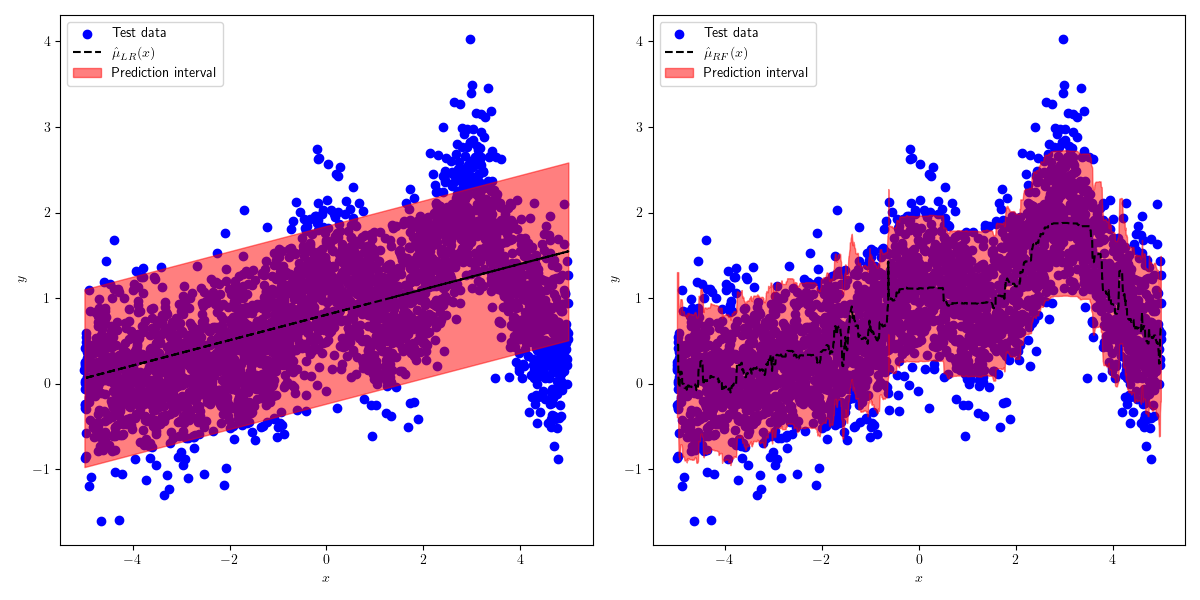
\includegraphics[width=\linewidth]{figures/2_3_LR_RF_example.png}
    \caption{Plot of the test data, the fitted regression function and the split conformal prediction interval using linear regression (left) and random forests (right). The fitted regression function is denoted \(\hat{\mu}_{LR}\)} (left) and \(\hat{\mu}_{RF}\) (right). \label{fig:split_LR_RF}
\end{figure}

\subsection{Choice of conformity score}
\label{subsec:conformityscore}

In \cref{subsec:splitconformal}, we showed that any conformity score can be used to construct the split conformal prediction set \eqref{eqn:split_absolute_residual_prediction_set}. However, it is not immediately clear from \eqref{eqn:split_absolute_residual_prediction_set} how the choice of conformity score affects the prediction set. We gain some insight into this from \cref{example:splitCP_absolute_residual_score}, where we see that for split conformal prediction with the absolute residual score, the conformity score influences the width of the prediction interval \textcolor{red}{through the quantile}. In this subsection, we further explore how the choice of conformity score affects the properties of the resulting prediction set. In addition to the absolute residual score, we consider two further examples of conformity scores in the regression setting and compare them through numerical experiments. Throughout this subsection, we use split conformal prediction.

\subsubsection{Regression}

We work in the regression setting as in \cref{example:splitCP_absolute_residual_score} with \(\mathcal{X} = \mathbb{R}\). Consider the absolute residual score and its corresponding predicition interval \eqref{eqn:split_absolute_residual_prediction_set}. We observe that a consequence of using the absolute residual score is that the prediction interval has a constant width for all \(x \in \mathbb{R}.\) If the data generating process is heteroscedastic, i.e. \(\R{Var}(Y | X = x)\) is not constant in \(x\), then the prediction interval \eqref{eqn:split_absolute_residual_prediction_set} does not accurately capture the uncertainty in \(Y\) given \(X = x\). This is closely related to the fact that \cref{thm:splitconformal_coverage} only guarantees \textit{marginal coverage} \[\Prob{Y_{n+1} \in C(X_{n+1}) } \geq 1-\alpha\] as opposed to \textit{test-conditional coverage} \[\Prob{Y_{n+1} \in C(X_{n+1}) \, | \, X_{n+1} } \geq 1-\alpha.\] This means that conformal prediction does not guarantee \(1-\alpha\) level coverage at every \(x \in \mathcal{X}\), but rather only on average over \(x\). The two conformity scores we present aim to make the prediction interval adaptive to heteroscedasticity. 

\subsubsection{Locally Weighted Residual Score}

If \(\hat{\mu}\) is an estimate of the regression function \(\mu:x \mapsto \Exp{Y | X = x}{(}{)}\) and \(\hat{\sigma}\) is an estimate of the \textit{conditional mean absolute deviation} \(x \mapsto \Exp{|Y-\mu(X)| \, \mid X = x}{(}{)}\), then the \textit{locally weighted score} is the conformity score given by \begin{equation}
    \hat{s}(x,y) = \frac{| y - \hat{\mu}(x)|}{\hat{\sigma}(x)}.
\end{equation} The corresponding prediction set is given by \begin{equation}
    C(x) = \left[ \hat{\mu}(x) - \hat{\sigma}(x) \, \hat{Q}_{(\hat{S}_1, \ldots, \hat{S}_n, \infty)}(1-\alpha), \ \hat{\mu}(x) + \hat{\sigma}(x) \, \hat{Q}_{(\hat{S}_1, \ldots, \hat{S}_n, \infty)}(1-\alpha) \right],
\end{equation} using the notation of \cref{subsec:splitconformal}. \vskip5pt

\noindent
This conformity score was originally introduced in \cite{lei2018} and aims to account for heteroscedasticity but scaling the width of the interval in \eqref{eqn:split_absolute_residual_prediction_set} by \(\hat{\sigma}(x)\) for each \(x \in \mathcal{X}\). In practice, \(\hat{\sigma}\) can be estimated by first regressing \(Y_i\) onto \(X_i\) for \((X_i, Y_i) \in D_\R{tr}\) to obtain \(\hat{\mu}\) and then regress \(|Y_i -\hat{\mu}(X_i)|\) onto \(X_i\) for \((X_i, Y_i) \in D_\R{tr}\).

\subsubsection{Conformalised Quantile Regression}

A second approach to generate prediction intervals that are adaptive to heteroscedasticity is to estimate the conditional quantile function \begin{equation}
    q_{\tau}(x) = \inf \left\{ z \in \mathbb{R}: \Prob{Y \leq z | X = x} \geq \tau \right\}, \quad \tau \in (0,1)
\end{equation} directly. This is motivated by noting that \[\Prob{Y \in [q_{\alpha/2}(X), q_{1-\alpha/2}(X)] \ | \  X} = 1-\alpha,\] i.e. the interval \([q_{\alpha/2}(X), q_{1-\alpha/2}(X)]\) has exact \((1-\alpha)-\)level test-conditional coverage. The approach of estimating \(q_\tau(x)\) is referred to as \textit{quantile regression}. In this essay, we do not discuss details of the numerous methods for constructing quantile regression estimators. However, we note that the following important fact. \vskip5pt

\noindent
Define the \(\tau-\)\textit{pinball loss} by \(\ell(y, y') = \rho_\tau(y - y')\), where \[\rho_\tau(u) = u(\tau - \Ind{u < 0} ) = \begin{cases}
    u\tau &\quad \text{if } u \geq 0, \\
    u(\tau - 1) &\quad \text{otherwise.}
\end{cases}\]

\begin{lemma}
    Let \(U\) be a real-valued random variable with density \(f\) and strictly increasing cumulative distribution function \(F\). Then for all \(\tau \in (0,1)\), we have that \[F^{-1}(\tau) = \argmin_{t \in \mathbb{R}} \Exp{\ell(Y,t)}{(}{)}\] 
\end{lemma}
\begin{proof}
    We have that \begin{align*}
        \Exp{\ell(Y,t)}{(}{)} = \Exp{\rho_\tau(Y-t)}{(}{)} &= \int_{-\infty}^\infty \rho_\tau(y-t) f(y) \, \R{d}y \\
        &= \int_{-\infty}^t (\tau-1) (y-t) f(y) \, \R{d}y + \int_t^\infty \tau(y-t) f(y) \, \R{d}y.
    \end{align*}
    Equating the derivative of the above expression with respect to \(t\) to \(0\) gives \[\int_{-\infty}^t (1-\tau) f(y) \, \R{d}y - \int_t^\infty \tau f(y) \, \R{d}y = (1-\tau)F(t) - \tau(1-F(t))  =  0,\] which is equivalent to \[t = F^{-1}(\tau).\] The second derivative is equal to \(f(t)\), so \(F^{-1}(\tau)\) is indeed a minimiser.
\end{proof}

\noindent
Therefore, in the same way that training a model with respect to the least-squares loss gives an estimate for the conditional mean, training a model with respect to the \(\tau-\)pinball loss gives an estimate of the \(\tau^{\R{th}}\) quantile of the conditional distribution \(Y|X\). \vskip5pt

\noindent
Using a quantile regression procedure, we may obtain estimates \(\hat{q}_{\alpha/2}(x)\) and \(\hat{q}_{1-\alpha/2}(x)\) for \(q_{\alpha/2}(x)\) and \(q_{1-\alpha/2}(x)\), respectively. However, the interval \([\hat{q}_{\alpha/2}(x), \hat{q}_{1-\alpha/2}(x)]\) may not be guaranteed to have \((1-\alpha)-\)level coverage in finite samples. \textit{Conformalised quantile regression} \cite{romano2019_CQR} calibrates this interval using conformal prediction to provide it with a finite-sample coverage guarantee as in \cref{thm:splitconformal_coverage}. \vskip5pt

\noindent
After obtaining estimates \(\hat{q}_{\alpha/2}(x)\) and \(\hat{q}_{1-\alpha/2}(x)\) from the proper training set, conformalised quantile regression applies split conformal prediction with the conformity score \begin{equation}
    \hat{s}(x,y) = \max\left\{ \hat{q}_{\alpha/2}(x) - y, \, y - \hat{q}_{1-\alpha/2}(x) \right\}.
\label{eqn:CQR_conformity_score}
\end{equation} This results in the conformal prediction interval \begin{align}
    &\left\{ y \in \mathbb{R}: \hat{q}_{\alpha/2}(X_{n+1}) - y \leq \hat{Q}_{(\hat{S}_1, \ldots, \hat{S}_n, \infty)}(1-\alpha) \quad \R{and} \quad y - \hat{q}_{1-\alpha/2}(X_{n+1}) \leq \hat{Q}_{(\hat{S}_1, \ldots, \hat{S}_n, \infty)}(1-\alpha) \right\} \nonumber \\
    &= \left[\hat{q}_{\alpha/2}(X_{n+1}) - \hat{Q}_{(\hat{S}_1, \ldots, \hat{S}_n, \infty)}(1-\alpha), \hat{q}_{1-\alpha/2}(X_{n+1}) + \hat{Q}_{(\hat{S}_1, \ldots, \hat{S}_n, \infty)}(1-\alpha)  \right].
\end{align}

\noindent
To intuitively understand this score, we note the following. If \(y < \hat{q}_{\alpha/2}(x)\), i.e. \(y\) is below the predicted lower quantile, then \(\hat{s}(x,y) = |y - \hat{q}_{\alpha/2}(x)|\) is the absolute error compared to the predicted lower quantile. Similarly, if \(y > \hat{q}_{1-\alpha/2}(x)\), then \(\hat{s}(x,y) = |y - \hat{q}_{1-\alpha/2}(x)|.\) In both of these cases, \(\hat{s}(x,y) \geq 0\), indicating the interval \([\hat{q}_{\alpha/2}(x), \hat{q}_{1-\alpha/2}(x)]\) has failed to cover \(y\), and its value measures the magnitude of the error in the fitted model with respect to \((x,y)\). If \(\hat{q}_{\alpha/2}(x) < y < \hat{q}_{1-\alpha/2}(x)\), i.e. the interval \([\hat{q}_{\alpha/2}(x), \hat{q}_{1-\alpha/2}(x)]\) covers \(y\), then \(\hat{s}(x,y) < 0\) and \[\hat{s}(x,y) = \min \left\{ y - \hat{q}_{\alpha/2}(x), \, \hat{q}_{1-\alpha/2}(x) - y \right\},\] which may be interpreted as the smaller of the two "margins" by which the interval \([\hat{q}_{\alpha/2}(x), \hat{q}_{1-\alpha/2}(x)]\) covers \(y\). Note that this contrasts to the conformity scores we have seen previously, which could only take on non-negative values. We see from the above that if the estimated interval \([\hat{q}_{\alpha/2}(x), \hat{q}_{1-\alpha/2}(x)]\) overcovers, then conformalised quantile regression narrows the interval, and if the estimated interval undercovers, then conformalised quantile regression widens the interval.

\subsubsection{Numerical Experiments}

We now present numerical experiments designed to highlight that the locally weighted score and conformalised quantile regression are more adaptive to heteroscedasticity. We consider two data generating processes. Setting 1 generates i.i.d. data points with homoscedastic noise, and setting 2 generates i.i.d data points with heteroscedastic noise.
\begin{enumerate}[(i)]
    \item \textbf{Setting 1: } \begin{align*}
        X_1, X_2, \ldots &\overset{\R{i.i.d}}{\sim} \R{Uniform}(-5,5) \\
        \epsilon_1, \epsilon_2, \ldots &\overset{\R{i.i.d}}{\sim} \mathcal{N}(0,1) \\
        Y_i &= 1 - X_i + 2\epsilon_i. 
    \end{align*} for all \(i \in [n]\).
    \item \textbf{Setting 2: } \begin{align*}
        X_1, X_2, \ldots &\overset{\R{i.i.d}}{\sim} \R{Uniform}(-5,5) \\
        \epsilon_1, \epsilon_2, \ldots &\overset{\R{i.i.d}}{\sim} \mathcal{N}(0,1) \\
        Y_i &= 1 - X_i + \frac{1}{2}(|X_i| + 2)(\sin(2X_i) + 3/2) \, \epsilon_i
    \end{align*} for all \(i \in [n]\).    
\end{enumerate}

\noindent
In each setting, we generate independent proper training, calibration and test datasets, set \(\alpha = 0.1\) and generate conformal prediction intervals for the test dataset using the absolute residual score, the locally weighted residual score and conformalised quantile regression. \textcolor{red}{Further details on the exact implementation and the code are provided in the appendix.} In \cref{tab:2_4_settings1_2_results}, we record the empirical coverage and the average length of the prediction intervals calculated on the test dataset. In \cref{fig:2_4_homoscedastic} and \cref{fig:2_4_heteroscedastic}, we plot the prediction intervals obtained using these three methods. \vskip5pt

\noindent
We observe that all three methods provide the target coverage in both settings. This is guaranteed by the theoretical coverage guarantee for split conformal prediction in \cref{thm:splitconformal_coverage} since all the data points are i.i.d., and thus exchangeable. However, we clearly see in \cref{fig:2_4_heteroscedastic} that the width of the prediction intervals \(C(x)\) obtained using the locally weighted residual score and conformalised quantile regression vary with \(x\) to account for the heteroscedasticity. Since the absolute residual score generates prediction intervals whose width is constant (in \(x\)), we see in \cref{fig:2_4_heteroscedastic_RF} that these overcover in some regions and undercover in others. Therefore, the absolute residual score yields wider prediction intervals as compared to the other two methods, which can be seen in \cref{tab:2_4_settings1_2_results}. This is further emphasised in \cref{fig:2_4_local_cov_setting2}, where we estimate the conditional coverage \(\Prob{Y_{n+1} \in C(X_{n+1} ) | X_{n+1}}\) by dividing the covariate space \((-5,5)\) into smaller subintervals and calculating the empirical coverage for the test dataset on each subinterval. This plot demonstrates that the locally weighted score and conformalised quantile regression provide improved conditional coverage compared to the absolute residual score.

\begin{table}[h]
    \centering
    \renewcommand{\arraystretch}{1.2}
    \begin{tabular}{|c|c|p{1.5cm}|c|p{1.5cm}|c|c|}
        \hline
        & \multicolumn{2}{c|}{Absolute residual} & \multicolumn{2}{c|}{Locally weighted} & \multicolumn{2}{c|}{Conformalised quantile regression} \\
        \hline
        & Coverage & Average length & Coverage & Average length & Coverage & Average length \\
        \hline
        Setting 1 & 0.9010 & 6.616 & 0.9027 & 6.632 & 0.9017 & 6.712 \\
        Setting 2 & 0.9003 & 13.03 & 0.9063 & 11.58 & 0.9027 & 11.55 \\
        \hline
    \end{tabular}
    \caption{Empirical coverage and average length of the conformal prediction intervals on the test dataset}
    \label{tab:2_4_settings1_2_results}
\end{table}

\begin{figure}[H]
    \centering
    \begin{subfigure}{0.32\textwidth}
    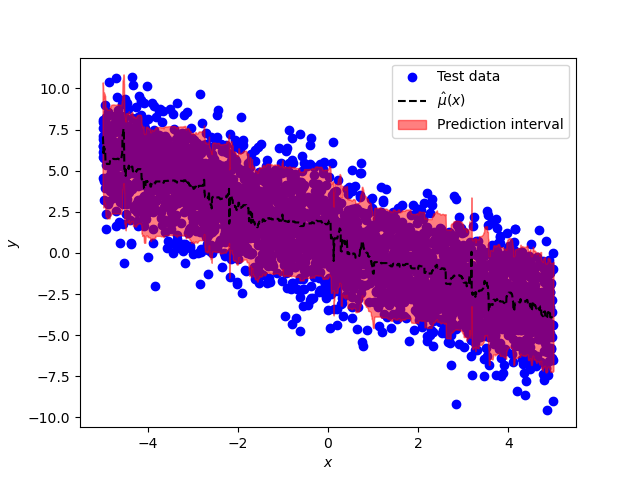
\includegraphics[width=\linewidth]{figures/2_4_homoscedastic_RF.png}    
    \caption{Absolute residual score} \label{fig:2_4_homoscedastic_RF}
    \end{subfigure}
    \begin{subfigure}{0.32\textwidth}
    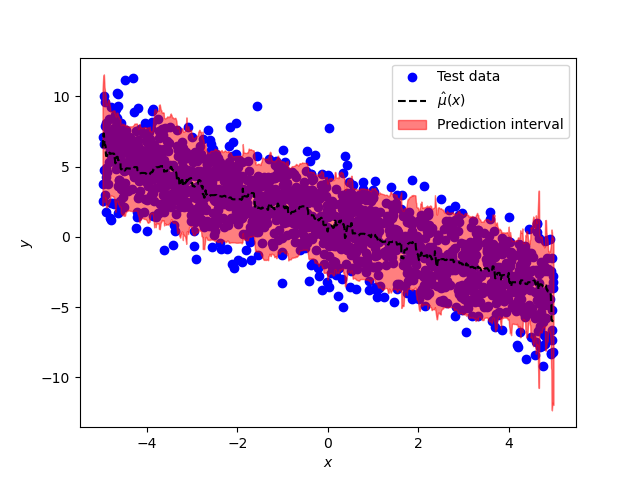
\includegraphics[width=\linewidth]{figures/2_4_homoscedastic_LW.png}
    \caption{Locally weighted score} \label{fig:2_4_homoscedastic_LW}
    \end{subfigure}
    \begin{subfigure}{0.32\textwidth}
    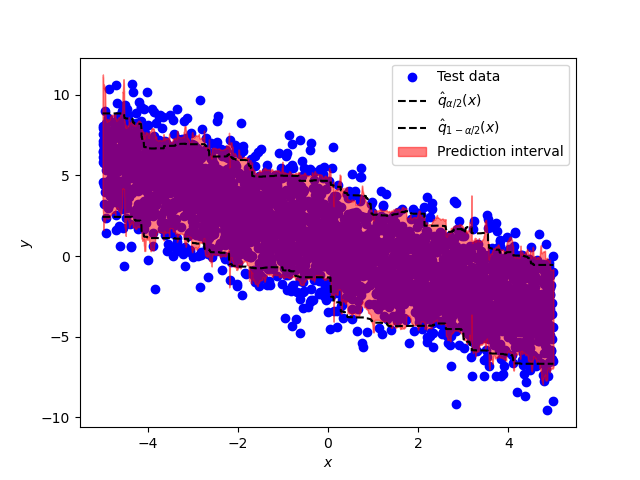
\includegraphics[width=\linewidth]{figures/2_4_homoscedastic_CQR.png}    
    \caption{Conformalised quantile regression} \label{fig:2_4_homoscedastic_CQR}
    \end{subfigure}
    \caption{Conformal prediction intervals in setting 1.}
\label{fig:2_4_homoscedastic}
\end{figure}

\begin{figure}[H]
    \centering
    \begin{subfigure}{0.45\textwidth}
    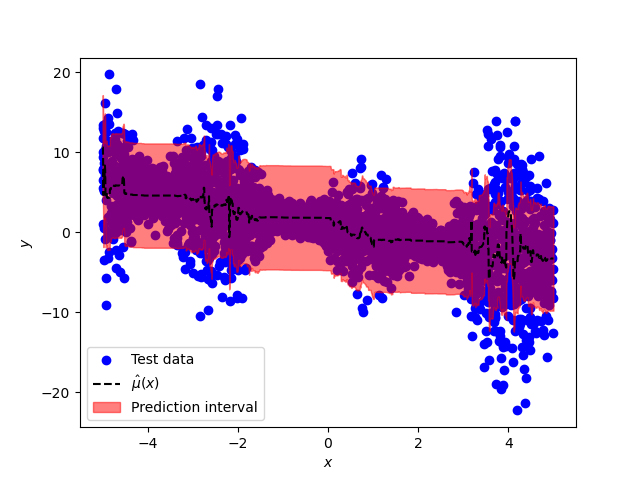
\includegraphics[width=\linewidth]{figures/2_4_heteroscedastic_RF.png}    
    \caption{Absolute residual score} \label{fig:2_4_heteroscedastic_RF}
    \end{subfigure}
    \begin{subfigure}{0.45\textwidth}
    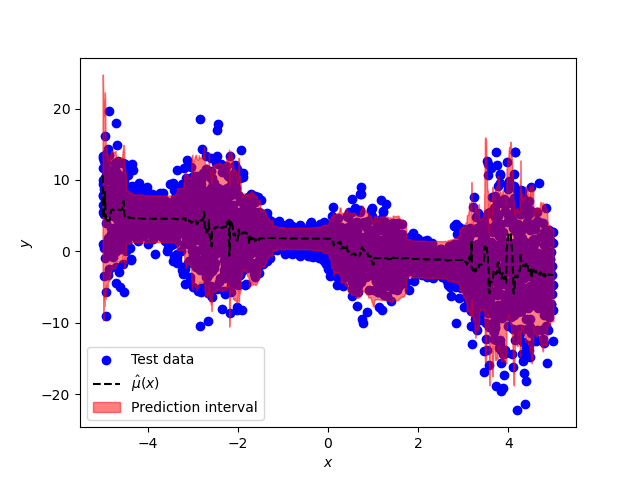
\includegraphics[width=\linewidth]{figures/2_4_heteroscedastic_LW.png}
    \caption{Locally weighted score} \label{fig:2_4_heteroscedastic_LW}
    \end{subfigure}
    \begin{subfigure}{0.45\textwidth}
    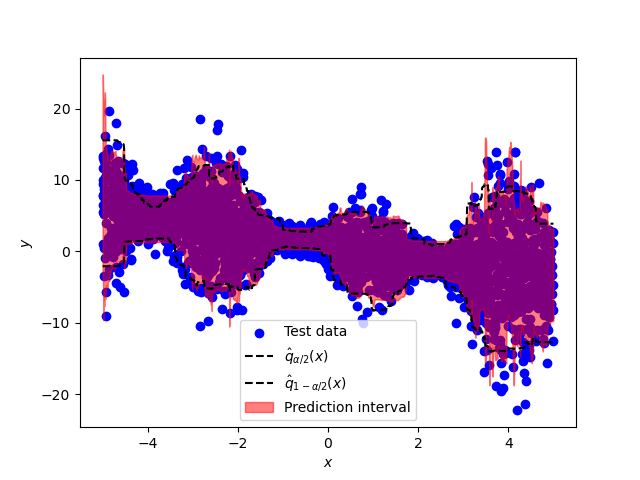
\includegraphics[width=\linewidth]{figures/2_4_heteroscedastic_CQR.png}    
    \caption{Conformalised quantile regression} \label{fig:2_4_heteroscedastic_CQR}
    \end{subfigure}
    \medskip
    \begin{subfigure}{0.45\textwidth}
    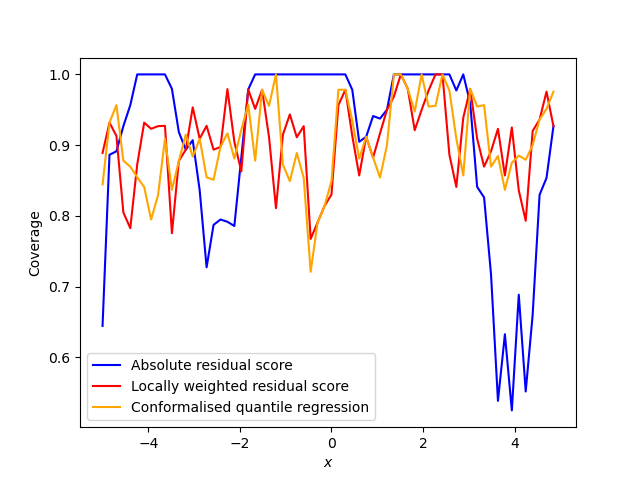
\includegraphics[width=\linewidth]{figures/2_4_local_cov_setting2.png}    
    \caption{Local coverage} \label{fig:2_4_local_cov_setting2}
    \end{subfigure}
    \caption{Conformal prediction intervals in setting 2.}
\label{fig:2_4_heteroscedastic}
\end{figure}


\section{Extensions of Conformal Prediction}

\subsection{Nonexchangeable Conformal Prediction}


In this subsection, we present the \textit{nonexchangeable conformal prediction} (NexCP) method developed in \cite{barber2023conformalbeyondexch}. In \cref{sec:foundations_of_CP}, we saw that the coverage guarantee of full conformal prediction relied on two key assumptions: the exchangeability of the data and the symmetry of the conformity score. \textcolor{red}{We saw that if the exchangeability assumption is violated, the coverage may deviate significantly from the target \(1-\alpha\) level.} The key theoretical contribution of \cite{barber2023conformalbeyondexch}, presented in \textcolor{red}{theorem ref}, is the development of a modified conformal prediction procedure where the loss of coverage due to violation of the above assumptions can be quantified. Furthermore, this result suggests empirical approaches to reduce this loss of coverage. \vskip5pt

\noindent
Before we present the main theorem of this subsection, we introduce the following notation. Given data points \((X_1, Y_1), \ldots, (X_{n+1}, Y_{n+1}) \in \mathcal{Z}\), \(y \in \mathcal{Y}\) and \(k \in [n+1]\), we define \[D = ((X_i, Y_i))_{i=1}^{n+1}, \quad D^{y} = ((X_i, Y_i)_{i=1}^n, (X_{n+1}, y)), \quad \quad D^{(k)} = \pi_k(D), \quad \mathrm{and} \quad D^{y, (k)} = \pi_k(D^{y}). \] where \(\pi_k \in S_{n+1}\) is the transposition exchanging \(k\) and \(n+1\). Given a conformity score \(s\), we additionally define \[S = (s((X_i, Y_i); D))_{i=1}^{n+1}, \quad \mathrm{and} \quad S^{(k)} = ( s(( X_{\pi_k(i)}, Y_{\pi_k(i)} ); D^{(k)}) )_{i=1}^{n+1}.\] We also define \[S_i^{y, (k)} = \begin{cases}
    s(( X_i, Y_i ); D^{y, (k)}) \quad &\mathrm{if} \ i = 1, \ldots, n \\
    s(( X_{n+1}, y ); D^{y, (k)}) \quad &\mathrm{if} \ i = n+1,
\end{cases} \quad \mathrm{and} \quad S^{y, (k)} = (S_i^{y,(k)})_{i=1}^{n+1}.\]

\noindent
We fix \textit{weights} \(w_1, \ldots, w_{n} \in [0, \infty)\) and correspondingly define \begin{equation}
    \tilde{w_i} = \frac{w_i}{1+\sum_{j=1}^n w_j} \quad \mathrm{and} \quad \tilde{w}_{n+1} = \frac{1}{1+\sum_{j=1}^n w_j}
\label{eqn:nexcp_weights_defn}
\end{equation} for all \(i \in [n]\). \vskip5pt

\noindent
We define \(K\) to be random variable taking values in \([n+1]\) such that \begin{equation}
    \Prob{K = k} = \tilde{w}_k
\label{eqn:nexcp_K_defn}
\end{equation} for all \(k \in [n+1]\), and we take \(K\) and \(D\) to be independent.

\begin{theorem}
    Let \((X_1, Y_1), \ldots, (X_{n+1}, Y_{n+1}) \in \mathcal{Z}\) be a sequence of tagged data points and \(s\) be a conformity score. Let \(w_1, \ldots, w_{n+1} \in [0, \infty)\) be fixed real numbers and define \(\tilde{w}_i\) according to \eqref{eqn:nexcp_weights_defn} for all \(i \in [n+1]\). Let \(K\) be a random variable as in \eqref{eqn:nexcp_K_defn} that is independent of \(D\). Define the prediction set \begin{equation}
        C(X_{n+1}) = \left\{ y \in \mathcal{Y} : \ S_{n+1}^{y, (K)} \leq \hat{Q}_{S^{y, (K)}}^{\tilde{w}}(1-\alpha)  \right\}.
    \label{eqn:nexcp_prediction_set}
    \end{equation} Then we have that \begin{equation}
        \Prob{Y_{n+1} \in C(X_{n+1})}  \geq 1-\alpha - \sum_{k=1}^n \R{d_{TV}}(S, S^{(k)}).
    \end{equation}
\label{thm:nexCP_coverage}
\end{theorem}
\begin{proof}
    If \(Y_{n+1} \not \in C(X_{n+1})\), then \[S_{n+1}^{Y_{n+1}, (K)} > \hat{Q}^{\tilde{w}}_{S_{n+1}^{Y_{n+1}, (K)}}(1-\alpha).\] This implies that \[S_{n+1}^{Y_{n+1}, (K)} > \hat{Q}^{\tilde{w}}_{\left( S_1^{Y_{n+1}, (K)}, \ldots, S_n^{Y_{n+1}, (K)}, \infty  \right)}(1-\alpha)\] by \textcolor{red}{cite lemma}. We now claim that \[\hat{Q}^{\tilde{w}}_{\left( S_1^{Y_{n+1}, (K)}, \ldots, S_n^{Y_{n+1}, (K)}, \infty  \right)}(1-\alpha) \geq \hat{Q}^{\tilde{w}}_{S^{(K)}}(1-\alpha).\] If \(K = n+1\), this is shown in the proof of \textcolor{red}{quantile lemma}. If \(K \leq n\), we have that for any \(x \in \mathbb{R}\), \begin{align*}
        \hat{F}^{\tilde{w}}_{S^{(K)}}(x) &= \sum_{i=1}^{n+1} \tilde{w}_i \Ind{x \geq S_{\pi_K(i)}^{Y_{n+1}, (K)}} \\
        &= \sum_{\substack{i = 1 \\ i \neq K}}^{n} \tilde{w}_i \Ind{x \geq S_i^{Y_{n+1}, (K)}} + \tilde{w}_K \Ind{x \geq S_{n+1}^{Y_{n+1}, (K)}} + \tilde{w}_{n+1} \Ind{x \geq S_K^{Y_{n+1}, (K)}} \\
        &= \hat{F}^{\tilde{w}}_{\left( S_1^{Y_{n+1}, (K)}, \ldots, S_n^{Y_{n+1}, (K)}, \infty  \right)}(x) + \tilde{w}_K \Ind{x \geq S_{n+1}^{Y_{n+1}, (K)}} + \tilde{w}_{n+1} \Ind{x \geq S_K^{Y_{n+1}, (K)}} \\
        & \hspace{4.8cm} -  \tilde{w}_K \Ind{x \geq S_{K}^{Y_{n+1}, (K)}} - \tilde{w}_{n+1} \Ind{x \geq \infty} \\
        &= \hat{F}^{\tilde{w}}_{\left( S_1^{Y_{n+1}, (K)}, \ldots, S_n^{Y_{n+1}, (K)}, \infty  \right)}(x) + \tilde{w}_K \left (\Ind{x \geq S_{n+1}^{Y_{n+1}, (K)}} - \Ind{x \geq \infty} \right) \\
        & \hspace{4.8cm} + \left( \tilde{w}_{n+1} - \tilde{w}_K\right) \left(\Ind{x \geq S_{K}^{Y_{n+1}, (K)}} - \Ind{x \geq \infty} \right) \\
        & \geq \hat{F}^{\tilde{w}}_{\left( S_1^{Y_{n+1}, (K)}, \ldots, S_n^{Y_{n+1}, (K)}, \infty  \right)}(x).
    \end{align*}
    Therefore, we have that \[\hat{F}^{\tilde{w}}_{S^{(K)}}\left( \hat{Q}^{\tilde{w}}_{\left( S_1^{Y_{n+1}, (K)}, \ldots, S_n^{Y_{n+1}, (K)}, \infty  \right)}(1-\alpha) \right) \geq 1-\alpha,\] by \textcolor{red}{basic lemma on quantiles} which shows the claim above. \vskip5pt

    \noindent
    So far, we have shown that \[Y_{n+1} \not \in C(X_{n+1}) \implies S_{n+1}^{Y_{n+1}, (K)} >\hat{Q}^{\tilde{w}}_{S^{(K)}}(1-\alpha).\] Noting that \(S_{n+1}^{Y_{n+1}, (K)} = S_K^{(K)}\), this implies that \[\Prob{Y_{n+1} \in C(X_{n+1}) } \geq 1 - \Prob{ S_K^{(K)} > \hat{Q}^{\tilde{w}}_{S^{(K)}}(1-\alpha) }. \]
    \noindent
    For \(r \in \mathbb{R}^{n+1}\), define \[\mathcal{S}(r) = \left\{ i \in [n+1]: \ r_i > \hat{Q}^{\tilde{w}}_r(1-\alpha) \right\}.\] Note that for any \(r \in \mathbb{R}^{n+1}\), \begin{align*}
        \sum_{i \in \mathcal{S}(r)} \tilde{w}_i &= \sum_{i=1}^{n+1} \tilde{w}_i \Ind{r_i > \hat{Q}^{\tilde{w}}_r(1-\alpha)} \\
        &= \sum_{i=1}^{n+1} \tilde{w}_i \Ind{\sum_{j=1}^{n+1} \tilde{w_j} \Ind{r_j < r_i} \geq 1-\alpha} \\
        &= \sum_{i=1}^{n+1} \tilde{w}_i \Ind{\sum_{j=1}^{n+1} \tilde{w_j} \Ind{r_i \leq r_j} \leq \alpha} \leq \alpha
    \end{align*} by \cref{lemma:harrison_2012}. \vskip5pt
    
    \noindent
    Thus, we have that \begin{align*}
        \Prob{ S_K^{(K)} > \hat{Q}^{\tilde{w}}_{S^{(K)}}(1-\alpha) } &= \Prob{K \in \mathcal{S}(S^{(K)})} \\
        &= \sum_{k=1}^{n+1} \tilde{w}_k \Prob{k \in \mathcal{S}(S^{(k)})} \\
        &= \sum_{k=1}^{n+1} \tilde{w}_k \Prob{k \in \mathcal{S}(S)} + \sum_{k=1}^{n+1} \tilde{w}_k \left[\Prob{k \in \mathcal{S}(S^{(k)})} - \Prob{k \in \mathcal{S}(S)} \right] \\
        &= \Exp{\sum_{k \in \mathcal{S}(S)} \tilde{w}_k }{[}{]} + \sum_{k=1}^{n} \tilde{w}_k \left[\Prob{k \in \mathcal{S}(S^{(k)})} - \Prob{k \in \mathcal{S}(S)} \right] \\
        &\leq \alpha + \sum_{k=1}^n \tilde{w}_k \, \R{d_{TV}}(S, S^{(k)}),
    \end{align*} where the second equality follows from the independence of \(K\) and the data, we use the result above and we note that \(S^{(n+1)} = S\). Overall, we deduce that \[\Prob{Y_{n+1} \in C(X_{n+1})}  \geq 1-\alpha - \sum_{k=1}^n \R{d_{TV}}(S, S^{(k)}).\]

\end{proof}


\subsection{Covariate Shift}


%This is how you can start a new page
\vfill \eject

%%%%%%%%%%%%%%%%%%%%%%%%%%%%%%%%%%%%%%%%%%%%%%%%%%%%%%%%%%%%%%%%%%%%%%
%                                                                             
% REFERENCES
%                                                                             
%%%%%%%%%%%%%%%%%%%%%%%%%%%%%%%%%%%%%%%%%%%%%%%%%%%%%%%%%%%%%%%%%%%%%%

% List any references you have used below. You can list papers in your preferred style, e.g. as below.
% To cite a paper in your text, use \cite{}.

\nocite{*}
\printbibliography

% If you prefer, you can list your papers in a separate .bib file. This is often much more efficient and easier to change later.
% An explanation of how to do this can be found at https://www.overleaf.com/learn/latex/Bibliography_management_with_bibtex.
% When submitting the essay, you must upload your .bib file alongside this .tex file.

\end{document}